% Compile with pdflatex. Each tikzpicture is one page, exported as rr-NAME.svg.
\documentclass[tikz,multi=tikzpicture,border=3pt]{standalone}
\usepackage{amsmath,lmodern}
\usetikzlibrary{arrows.meta,calc}
\definecolor{ink}{HTML}{263943}
\definecolor{accent}{HTML}{205F72}
\definecolor{guide}{HTML}{586A73}
\definecolor{wash}{HTML}{E4F0F3}
\tikzset{every picture/.style={x=1cm,y=1cm,draw=ink,text=ink,font=\small,
    line width=.78pt,line cap=round,line join=round,>=Stealth},
    trace/.style={draw=accent,line width=1.1pt},
    motion/.style={trace,-{Stealth[length=2.4mm,width=1.8mm]}},
    axis/.style={draw=guide,line width=.55pt,-{Stealth[length=1.8mm]}},
    hidden/.style={draw=guide,dash pattern=on 2pt off 2.2pt,line width=.5pt},
    dim/.style={draw=guide,|-|,thin}, every node/.style={inner sep=1.5pt}}
\newcommand{\sheet}{\path[use as bounding box] (-.12,-.22) rectangle (7.12,4.24);}
\newcommand{\pt}[1]{\fill[ink] #1 circle[radius=1.8pt];}
\begin{document}
% parabola
\begin{tikzpicture}
\sheet
\begin{scope}[shift={(.86,.46)},x=1.02cm,y=.210cm]
\draw[axis] (-.2,0)--(5.55,0) node[right]{$x$};
\draw[axis] (0,-.25)--(0,17.1) node[left]{$y$};
\draw[hidden] (0,9) node[left]{$9$}--(3,9)--(3,0) node[below]{$3$};
\draw[trace,domain=0:3.98,samples=70] plot(\x,{\x*\x});
\draw[motion,domain=2.04:2.51,samples=15] plot(\x,{\x*\x});
\pt{(3,9)} \node[right=4pt] at (3,9) {$(3,9)$};
\node[text=accent] at (4.95,15.6) {$y=x^2$};
\end{scope}
\end{tikzpicture}
% circle
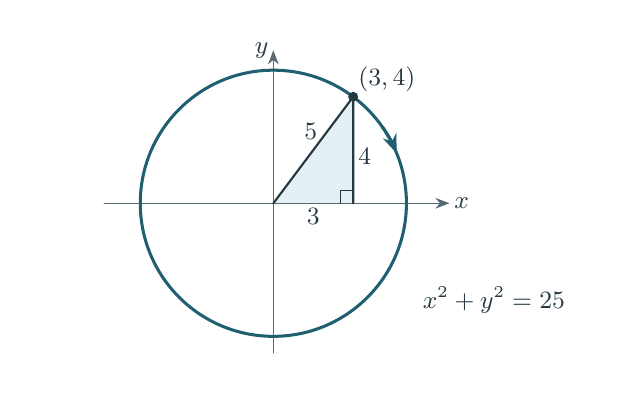
\begin{tikzpicture}
\sheet
\begin{scope}[shift={(3.0,2.01)},x=.338cm,y=.338cm]
\fill[wash] (0,0)--(3,0)--(3,4)--cycle;
\draw[axis] (-6.35,0)--(6.62,0) node[right]{$x$};
\draw[axis] (0,-5.62)--(0,5.75) node[left]{$y$};
\draw[trace] (0,0) circle[radius=1.69cm];
\draw (0,0)--(3,4) node[pos=.58,above left=-1pt]{$5$}--(3,0);
\draw[thin] (2.52,0)--(2.52,.48)--(3,.48);
\node[below] at (1.5,0) {$3$}; \node[right] at (3,1.75) {$4$};
\pt{(3,4)} \node[above right] at (3,4) {$(3,4)$};
\draw[motion] (35:5) arc[start angle=35,end angle=22,radius=5];
\end{scope}
\node at (5.8,.78) {$x^2+y^2=25$};
\end{tikzpicture}
% hyperbola
\begin{tikzpicture}
\sheet
\begin{scope}[shift={(.77,.42)},x=.72cm,y=.43cm]
\draw[axis] (-.18,0)--(8.15,0) node[right]{$x$};
\draw[axis] (0,-.16)--(0,8.32) node[left]{$y$};
\draw[hidden] (0,4) node[left]{$4$}--(3,4)--(3,0) node[below]{$3$};
\draw[trace,domain=1.55:7.93,samples=90] plot(\x,{12/\x});
\draw[motion,domain=4.25:5.1,samples=16] plot(\x,{12/\x});
\pt{(3,4)} \node[above right] at (3,4) {$(3,4)$};
\node[text=accent] at (6,6.3) {$xy=12$};
\end{scope}
\end{tikzpicture}
% balloon
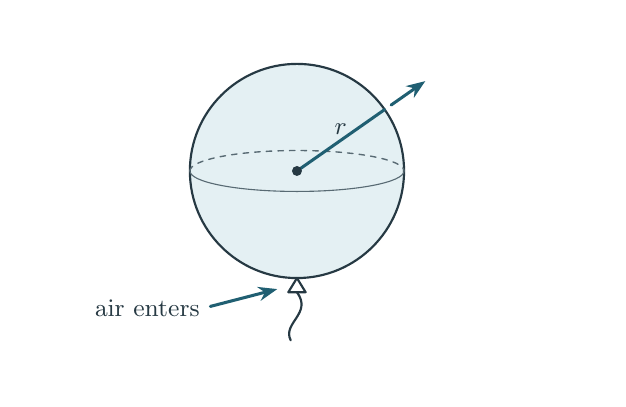
\begin{tikzpicture}
\sheet
\coordinate (C) at (3.3,2.42);
\draw[fill=wash] (C) circle (1.36);
\draw[hidden] (1.94,2.42) arc[start angle=180,end angle=0,x radius=1.36,y radius=.26];
\draw[thin,guide] (1.94,2.42) arc[start angle=180,end angle=360,x radius=1.36,y radius=.26];
\draw[trace] (C)--++(35:1.36) node[midway,above]{$r$}; \pt{(C)}
\draw[motion] ($(C)+(35:1.46)$)--++(35:.53);
\draw (3.3,1.06)--(3.19,.88)--(3.41,.88)--cycle;
\draw (3.3,.88) .. controls (3.5,.61) and (3.11,.49) .. (3.22,.27);
\node[left] at (2.13,.68) {air enters}; \draw[motion] (2.20,.7)--(3.05,.92);
\end{tikzpicture}
% cube
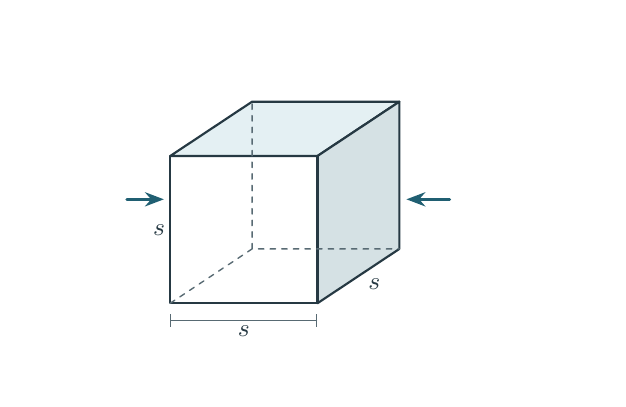
\begin{tikzpicture}
\sheet
\coordinate (A) at (1.69,.74);
\begin{scope}[shift={(A)}]
\draw[fill=wash] (0,1.87)--(1.04,2.56)--(2.91,2.56)--(1.87,1.87)--cycle;
\draw[fill=accent!19] (1.87,0)--(2.91,.69)--(2.91,2.56)--(1.87,1.87)--cycle;
\draw (0,0) rectangle (1.87,1.87);
\draw[hidden] (0,0)--(1.04,.69)--(2.91,.69) (1.04,.69)--(1.04,2.56);
\draw[dim] (0,-.22)--(1.87,-.22) node[midway,below]{$s$};
\node[left] at (0,.93) {$s$}; \node[below right] at (2.45,.38) {$s$};
\draw[motion] (-.55,1.32)--(-.08,1.32); \draw[motion] (3.55,1.32)--(3,1.32);
\end{scope}
\end{tikzpicture}
% rectangle
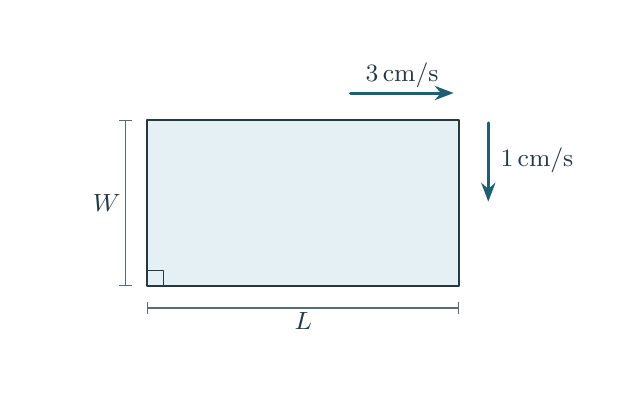
\begin{tikzpicture}
\sheet
\draw[fill=wash] (1.40,.96) rectangle (5.36,3.07);
\draw[thin] (1.4,1.16)--(1.60,1.16)--(1.60,.96);
\draw[dim] (1.4,.68)--(5.36,.68) node[midway,below]{$L$};
\draw[dim] (1.12,.96)--(1.12,3.07) node[midway,left]{$W$};
\draw[motion] (3.98,3.41)--(5.29,3.41) node[midway,above]{$3\,\mathrm{cm/s}$};
\draw[motion] (5.73,3.03)--(5.73,2.03);
\node[right] at (5.82,2.55) {$1\,\mathrm{cm/s}$};
\end{tikzpicture}
% triangle
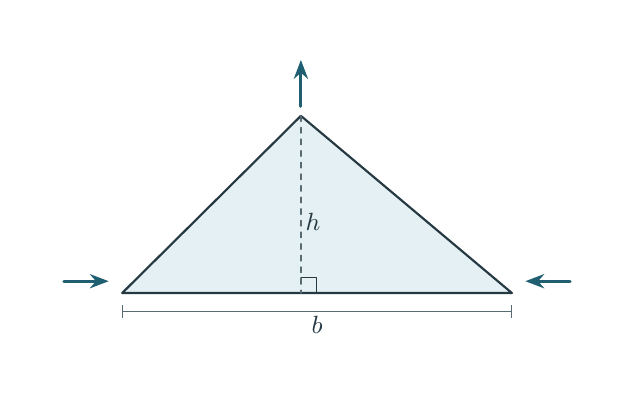
\begin{tikzpicture}
\sheet
\coordinate (A) at (1.08,.87); \coordinate (B) at (6.03,.87);
\coordinate (T) at (3.35,3.12); \coordinate (F) at (3.35,.87);
\draw[fill=wash] (A)--(T)--(B)--cycle;
\draw[hidden] (T)--(F) node[pos=.6,right]{$h$};
\draw[thin] (F)++(0,.20)--++(.20,0)--++(0,-.20);
\draw[dim] (1.08,.64)--(6.03,.64) node[midway,below]{$b$};
\draw[motion] (.34,1.02)--(.91,1.02); \draw[motion] (6.77,1.02)--(6.20,1.02);
\draw[motion] (3.35,3.24)--(3.35,3.83);
\end{tikzpicture}
% ladder
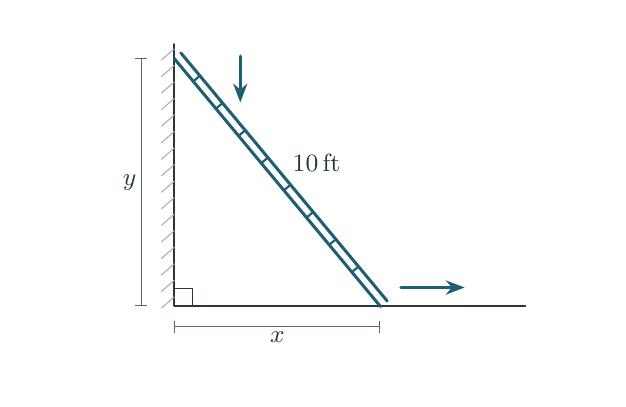
\begin{tikzpicture}
\sheet
\coordinate (B) at (4.36,.70); \coordinate (T) at (1.74,3.85);
\draw (1.74,4.03)--(1.74,.70)--(6.20,.70);
\foreach \y in {.82,1.03,...,3.99} \draw[thin,guide!52] (1.58,\y-.14)--(1.74,\y);
\draw[thin] (1.74,.93)--(1.97,.93)--(1.97,.70);
\begin{scope}[shift={(T)},rotate=-50.25]
\draw[trace] (0,0)--(4.10,0) (0,.11)--(4.10,.11);
\foreach \x in {.38,.83,...,3.87} \draw[accent] (\x,0)--(\x,.11);
\end{scope}
\node[above right] at (3.18,2.35) {$10\,\mathrm{ft}$};
\draw[dim] (1.32,.70)--(1.32,3.85) node[midway,left]{$y$};
\draw[dim] (1.74,.44)--(4.36,.44) node[midway,below]{$x$};
\draw[motion] (2.58,3.88)--(2.58,3.29);
\draw[motion] (4.62,.94)--(5.43,.94);
\end{tikzpicture}
% boat
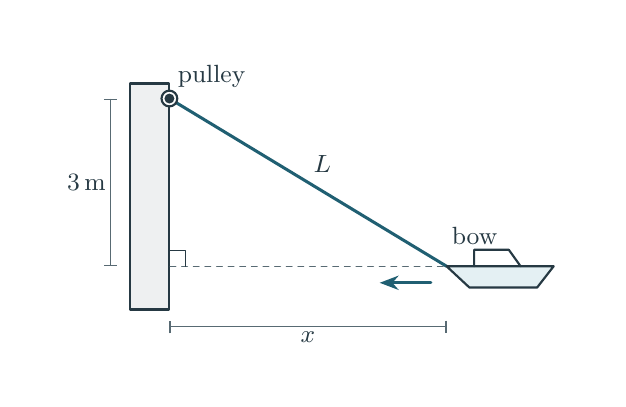
\begin{tikzpicture}
\sheet
\draw[fill=guide!10] (1.18,.66) rectangle (1.68,3.53);
\draw[hidden] (1.69,1.21)--(5.20,1.21);
\draw[trace] (1.68,3.34)--(5.20,1.21) node[pos=.49,above right=1pt]{$L$};
\draw[fill=white] (1.68,3.34) circle (.10); \pt{(1.68,3.34)}
\node[above right] at (1.72,3.42) {pulley};
\draw[thin] (1.68,1.41)--(1.88,1.41)--(1.88,1.21);
\draw[fill=wash] (5.20,1.21)--(5.49,.94)--(6.35,.94)--(6.56,1.21)--cycle;
\draw (5.55,1.21)--(5.55,1.42)--(5.99,1.42)--(6.14,1.21);
\node[right] at (5.20,1.59) {bow}; \draw[motion] (5.00,1.00)--(4.35,1.00);
\draw[dim] (.93,1.21)--(.93,3.34) node[midway,left]{$3\,\mathrm m$};
\draw[dim] (1.68,.44)--(5.20,.44) node[midway,below]{$x$};
\end{tikzpicture}
% cone
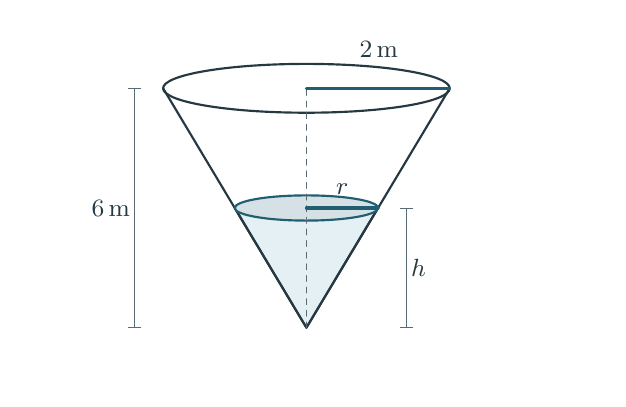
\begin{tikzpicture}
\sheet
\coordinate (V) at (3.42,.43);
\draw[fill=wash] (2.51,1.95)--(V)--(4.33,1.95)--cycle;
\draw (1.60,3.47)--(V)--(5.24,3.47);
\draw (3.42,3.47) ellipse (1.82 and .31);
\draw[accent,fill=accent!19] (3.42,1.95) ellipse (.91 and .16);
\draw[hidden] (V)--(3.42,3.47);
\draw[trace] (3.42,3.47)--(5.24,3.47);
\node at (4.34,3.96) {$2\,\mathrm m$};
\draw[trace] (3.42,1.95)--(4.33,1.95) node[midway,above=3pt]{$r$};
\draw[dim] (1.24,.43)--(1.24,3.47) node[midway,left]{$6\,\mathrm m$};
\draw[dim] (4.69,.43)--(4.69,1.95) node[midway,right]{$h$};
\end{tikzpicture}
% shadow
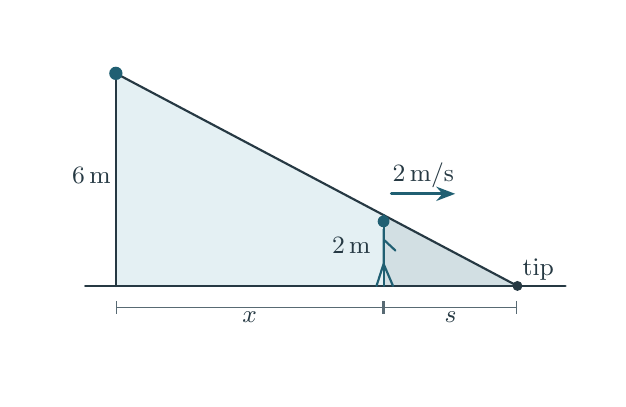
\begin{tikzpicture}
\sheet
\coordinate (L) at (1.0,3.66); \coordinate (P) at (4.40,1.86); \coordinate (E) at (6.10,.96);
\fill[wash] (1,.96)--(L)--(E)--cycle;
\fill[accent!20] (4.4,.96)--(P)--(E)--cycle;
\draw (0.61,.96)--(6.71,.96); \draw (1,.96)--(L);
\draw (L)--(E); \fill[accent] (L) circle (2.4pt); \pt{(E)}
\node[left] at (1,2.36) {$6\,\mathrm m$};
\draw[accent] (4.40,.96)--(P);
\fill[accent] (4.40,1.78) circle (.075);
\draw[accent] (4.40,1.68)--(4.40,1.24)--(4.31,.96) (4.40,1.24)--(4.52,.96) (4.40,1.55)--(4.55,1.41);
\node[left] at (4.30,1.48) {$2\,\mathrm m$};
\node[above right] at (E) {tip};
\draw[motion] (4.5,2.13)--(5.31,2.13) node[midway,above]{$2\,\mathrm{m/s}$};
\draw[dim] (1,.69)--(4.4,.69) node[midway,below]{$x$};
\draw[dim] (4.4,.69)--(6.10,.69) node[midway,below]{$s$};
\end{tikzpicture}
% similar
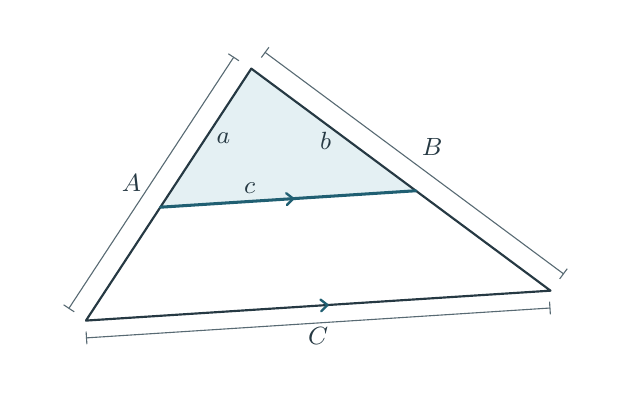
\begin{tikzpicture}
\sheet
\coordinate (A) at (2.72,3.72); \coordinate (B) at (.62,.52); \coordinate (C) at (6.52,.90);
\coordinate (b) at ($(A)!.55!(B)$); \coordinate (c) at ($(A)!.55!(C)$);
\fill[wash] (A)--(b)--(c)--cycle;
\draw[ink] (A)--(B)--(C)--cycle;
\draw[trace] (b)--(c);
% Identical chevrons mark the parallel sides.
\foreach \p/\q in {B/C,b/c}{
  \begin{scope}[shift={($(\p)!.52!(\q)$)},rotate=3.685]
    \draw[accent,line width=.85pt] (-.085,.075)--(0,0)--(-.085,-.075);
  \end{scope}
}
% Lowercase labels lie beside the small triangle's edges.
\path (A)--(b) node[midway,right=2pt] {$a$};
\path (A)--(c) node[midway,below left=-1pt] {$b$};
\path (b)--(c) node[pos=.35,above=1pt] {$c$};
% Dimension lines measure the full outer sides, including the shared portions.
\draw[dim] ($(B)+(-.22,.15)$)--($(A)+(-.22,.15)$) node[midway,left=2pt] {$A$};
\draw[dim] ($(A)+(.17,.21)$)--($(C)+(.17,.21)$) node[midway,above right=1pt] {$B$};
\draw[dim] ($(B)+(0,-.22)$)--($(C)+(0,-.22)$) node[midway,below] {$C$};
\end{tikzpicture}
\end{document}
